\begin{figure}[htbp]
\centering
\begin{tabular}{@{}c@{\hspace{8pt}}c@{\hspace{8pt}}c@{}}
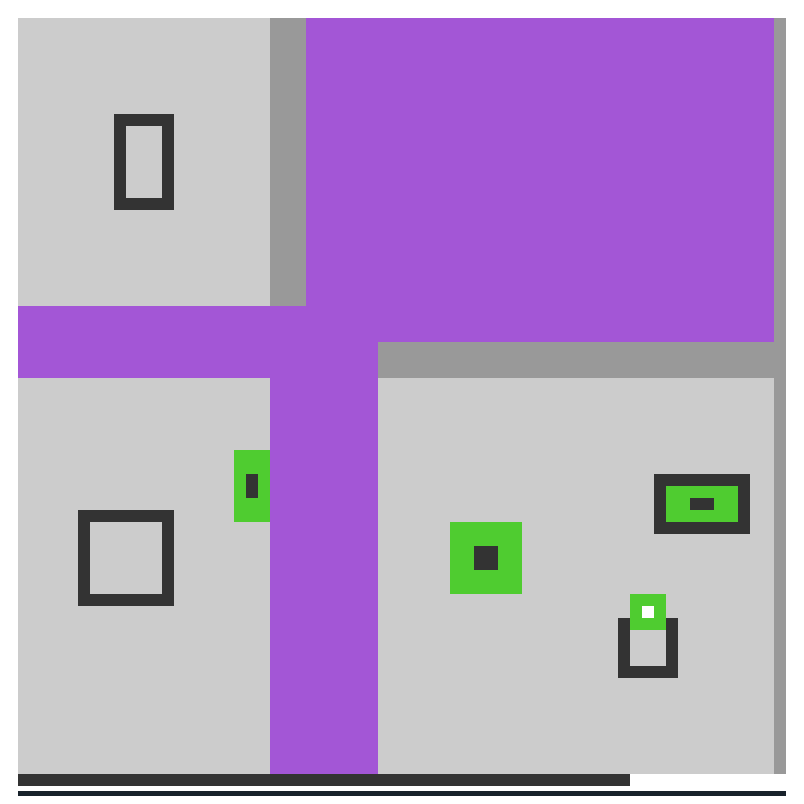
\includegraphics[width=0.29\linewidth]{figures/runs/step-counter-a.png} &
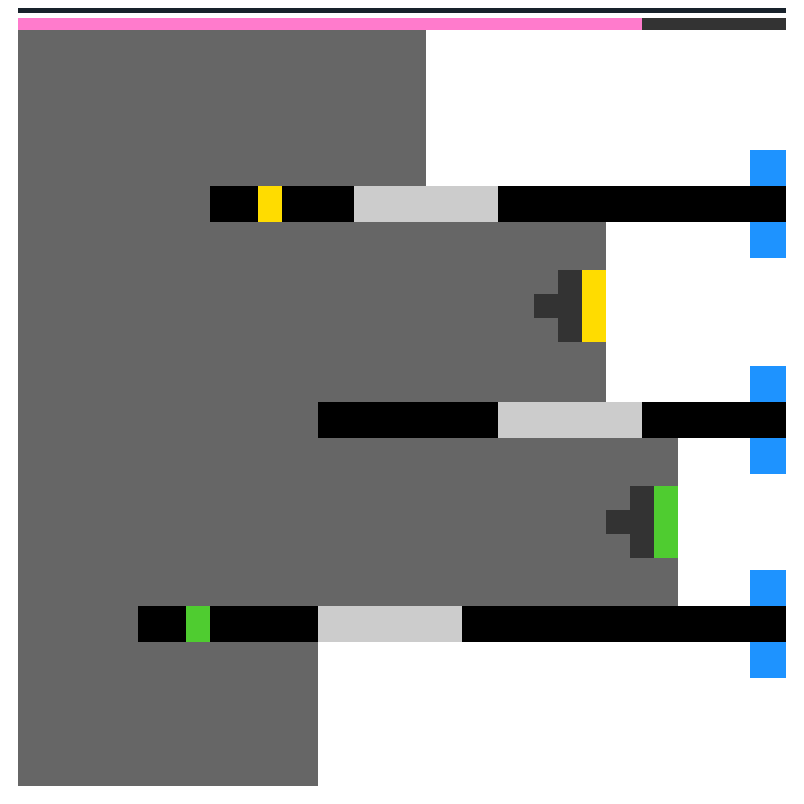
\includegraphics[width=0.29\linewidth]{figures/runs/step-counter-b.png} &
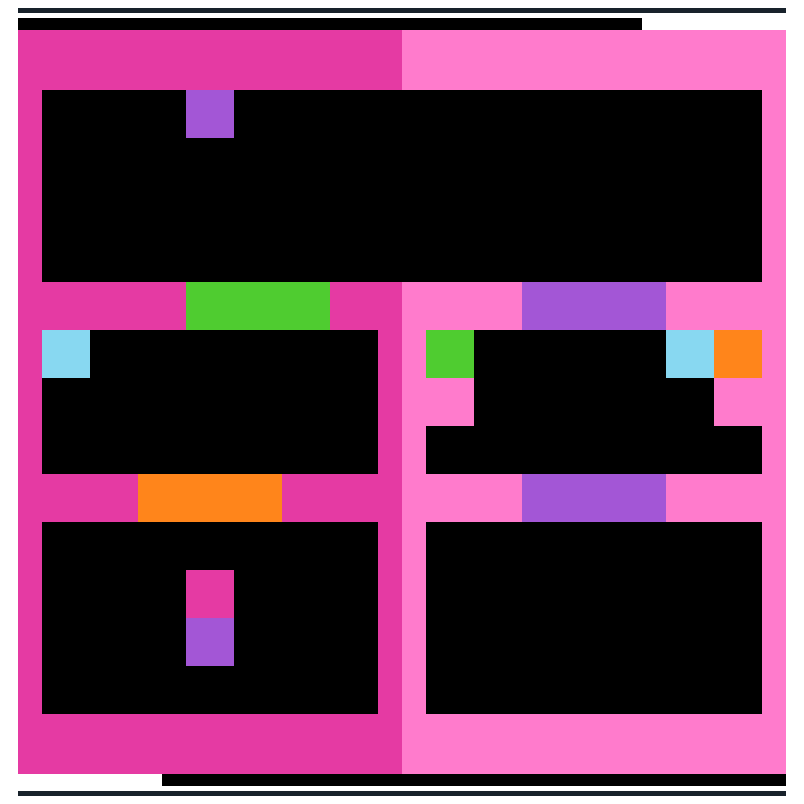
\includegraphics[width=0.29\linewidth]{figures/runs/step-counter-c.png}\\[1pt]
\footnotesize (a) \texttt{ka59}, level 2: bottom row & \footnotesize (b) \texttt{vc33}, level 5: top row & \footnotesize (c) \texttt{m0r0}, level 5: top and bottom rows
\end{tabular}\\[7pt]
\begin{tabular}{@{}r@{\hspace{8pt}}c@{}}
\footnotesize After action 30 & \raisebox{-0.3\height}{\board[0.74\linewidth]{step-counter-d.png}}\\[5pt]
\footnotesize After action 53 & \raisebox{-0.3\height}{\board[0.74\linewidth]{step-counter-e.png}}\\[5pt]
\footnotesize After action 77 & \raisebox{-0.3\height}{\board[0.74\linewidth]{step-counter-f.png}}
\end{tabular}\\[3pt]
{\footnotesize (d) Close-up of the bottom four rows in (a) at three points during level 2}
\caption{\textbf{Some games show a bar that changes as the agent takes actions.} These examples come from the evaluated layered runs. The bar is on the bottom row in (a), the top row in (b), and both the top and bottom rows in (c). The dark lines drawn outside the boards mark the cells the harness ignored when comparing boards. The figure adds these lines. Panel (d) shows a close-up of the bar in (a). Its dark section shrank from 63 cells after action 30 to 51 after action 53 and 39 after action 77. The harness can miss a counter, and some games have no visible counter \citep{dai2026runfigures}.}\label{fig:step-counter}
\end{figure}
